\documentclass{gmto}

\usepackage{amsmath}
\usepackage[load=accepted]{siunitx}
\usepackage{todonotes}

\DocID{GMT-XXX-\#\#\#\#}
\DocVersion{1.0}
\DocStatus{Draft}

\addbibresource{gmt.bib}

\title{Natural Seeing Observatory Performance Mode Integrated Model Description}
%\subtitle{}
\author{R. Conan, R. Romano, C. Dribusch, H. Fitzpatrick}
\date{\today}

\begin{document}

\maketitle

\clearpage

\section*{Signatures}
\vspace{1cm}
\subsection*{Author}
\vspace{1.5cm}
%\tabulinesep=1em
\begin{tabu} to \linewidth {X[3,l]X[1,l]}
  \rule{\linewidth}{.1pt} & \rule{\linewidth}{.1pt} \\
  Name, title & Date
\end{tabu}
\vspace{1.5cm}
\subsection*{Approvers}
\vspace{1.5cm}
%\tabulinesep=1em
\begin{tabu} to \linewidth {X[3,l]X[1,l]}
  \rule{\linewidth}{.1pt} & \rule{\linewidth}{.1pt} \\
  Name, title & Date \\[1cm]
  \rule{\linewidth}{.1pt} & \rule{\linewidth}{.1pt} \\
  Name, title & Date
\end{tabu}

\clearpage

\section*{Revision Log}

\begin{revisions}
  1.0 & \today & All & None & Initial version & Author \\  
\end{revisions}

\clearpage

\tableofcontents
\listoffigures
\listoftables

\clearpage

\section{Purpose}
\label{sec:purpose}

This document describe the GMT integrated model for the Natural Seeing
Observatory performance mode\cite{ORD}.

\section{Introduction}
\label{sec:introduction}

The integrated model is made of 3 main models of the telescope:
\begin{enumerate}
\item the finite element model of the telescope (FEM),
\item the optical model,
\item the control systems.
\end{enumerate}

In addition, other models are used to compute the disturbances applied to the
integrated model like the atmospheric turbulence model, the computational fluid
dynamics model that computes the dome seeing and the wind pressure exerted on
the telescope, the heat conjugate transfer model of M1 segments to compute the
segments thermal figure errors ...

\begin{figure}
  \centering
%  \includegraphics[width=\textwidth]{/home/rconan/Documents/GMT/Review/ASMFDR/nsiq.png}
  \caption{Natural Seeing image quality error budget.}
  \label{fig:ns-iq}
\end{figure}

\clearpage
\section{Models}
\label{sec:models}

\subsection{Finite element model}

The finite element model of the telescope\cite{ss2fem_Christoph2020} includes
the mount\cite{mount_pdr_iv} (pointing at a 60 degree elevation angle), M1 segments, M2
segments and the telescope pier.
The FEM is modeled as a set of second order ordinary differential
equations (ODE) relating nodal displacements, velocities and accelerations to
forces on the telescope.
The ODEs can be rewritten as a function of the eigen modes $\vec q$ of the telescope
FEM, the ODE of a given eigen mode $q_i$ is written:
\begin{equation}
  \label{eq:1}
  \ddot q_i + 2\omega_i\zeta\dot q_i + \omega_i^2 q_i = \vec b_i\cdot \vec u,
\end{equation}
where $\omega_i$ is the eigen frequency, $\zeta$ the damping coefficient, $\vec b_i$
the nodal to modal forces projection vector and $\vec u$ the vector of nodal forces.
The corresponding telescope nodal displacement $\vec y$ are derived from
\begin{equation}
  \label{eq:2}
  \vec y = \sum_i q_i\vec c_i  = \sum_i \vec y_i,
\end{equation}
where $\vec c_i$ is the modal to nodal displacement transformation vector.

The scalar ODE in Eq.~(\ref{eq:1}) is rewritten in the following state space model:
\begin{eqnarray}
  \label{eq:3}
  \dot x_i &=& A_ix_i + B_iu   \\
  y_i &=& C_ix_i,
\end{eqnarray}
with
$$
x_i = \begin{bmatrix}
    q_i \\
    \dot q_i
    \end{bmatrix},
  A_i = \begin{bmatrix}
    0 & 1 \\
    -\omega_i^2 & -2\omega_i\zeta
    \end{bmatrix}  
    ,
    B_i = \begin{bmatrix}
      \vec 0 \\
      \vec b
      \end{bmatrix}
    ,
    C_i = \begin{bmatrix}
      \vec c_i & \vec 0
    \end{bmatrix}
    .
$$
  The continuous state space model is transformed into a discrete state space model
  \begin{eqnarray}
    \label{eq:4a}
  x_i[k+1] &=& A_{i,d} x[k] + B_{i,d} u[k] \\
    \label{eq:4b}
  y_i[k] &=& C_i x_i[k],
  \end{eqnarray}
  with
  $$
  A_{i,d} = \exp(A_i\tau),
   B_{i,d} = A_i^{-1}(A_{i,d}-I)B_i$$
  and $\tau$ is the sample time.
Both $A_{i,d}$\footnote{\url{https://www.wolframalpha.com/input/?i=inverse+\%7B\%7B0\%2C+1\%7D\%2C+\%7B-x\%5E2\%2C+-2yx\%7D\%7D}} and $A_i^{-1}$\footnote{\url{https://www.wolframalpha.com/input/?i=Matrixexp\%5B\%7B\%7B0\%2Ct\%7D\%2C\%7B-tx\%5E2\%2C-2txy\%7D\%7D\%5D}} have a closed-form expression:
\begin{equation}
  \label{eq:5}
  A_{i,d} = \begin{bmatrix}
    {\alpha_+\beta_- + \alpha_-\beta_+ \over 2z_i} & {\beta_- - \beta_+ \over 2z_i} \\
    {\omega_i^2 (\beta_+ - \beta_-) \over 2z_i} & {\alpha_-\beta_- + \alpha_+\beta_+ \over 2z_i}
    \end{bmatrix}
\end{equation}
\begin{equation}
  \label{eq:6}
  A_i^{-1} = \begin{bmatrix}
    -2\zeta\omega_i^{-1} & -\omega_i^{-2} \\
    1 & 0
  \end{bmatrix}  
\end{equation}
with $z_i=\omega_i^2\sqrt{\zeta^2-1}$, $\alpha_-=z_i-\omega_i\zeta$,
$\alpha_+=z_i+\omega_i\zeta$, $\beta_-=\exp(\tau\alpha_-)$,
$\beta_+=\exp(-\tau\alpha_+)$.
Thanks to the orthogonality of the eigen modes $q_i$, the discrete state space
models given by Eq.~(\ref{eq:4a}) and Eq.~(\ref{eq:4b}) are computed in parallel  for all the modes of
the system.

The eigen modes of the telescope FEM\cite{} have been computed for all the modes
up to a eigen frequency of 2,000Hz leading to a total of 13,381 modes(Fig.~\ref{fig:fem-eig-val}).
\begin{figure}
  \centering
  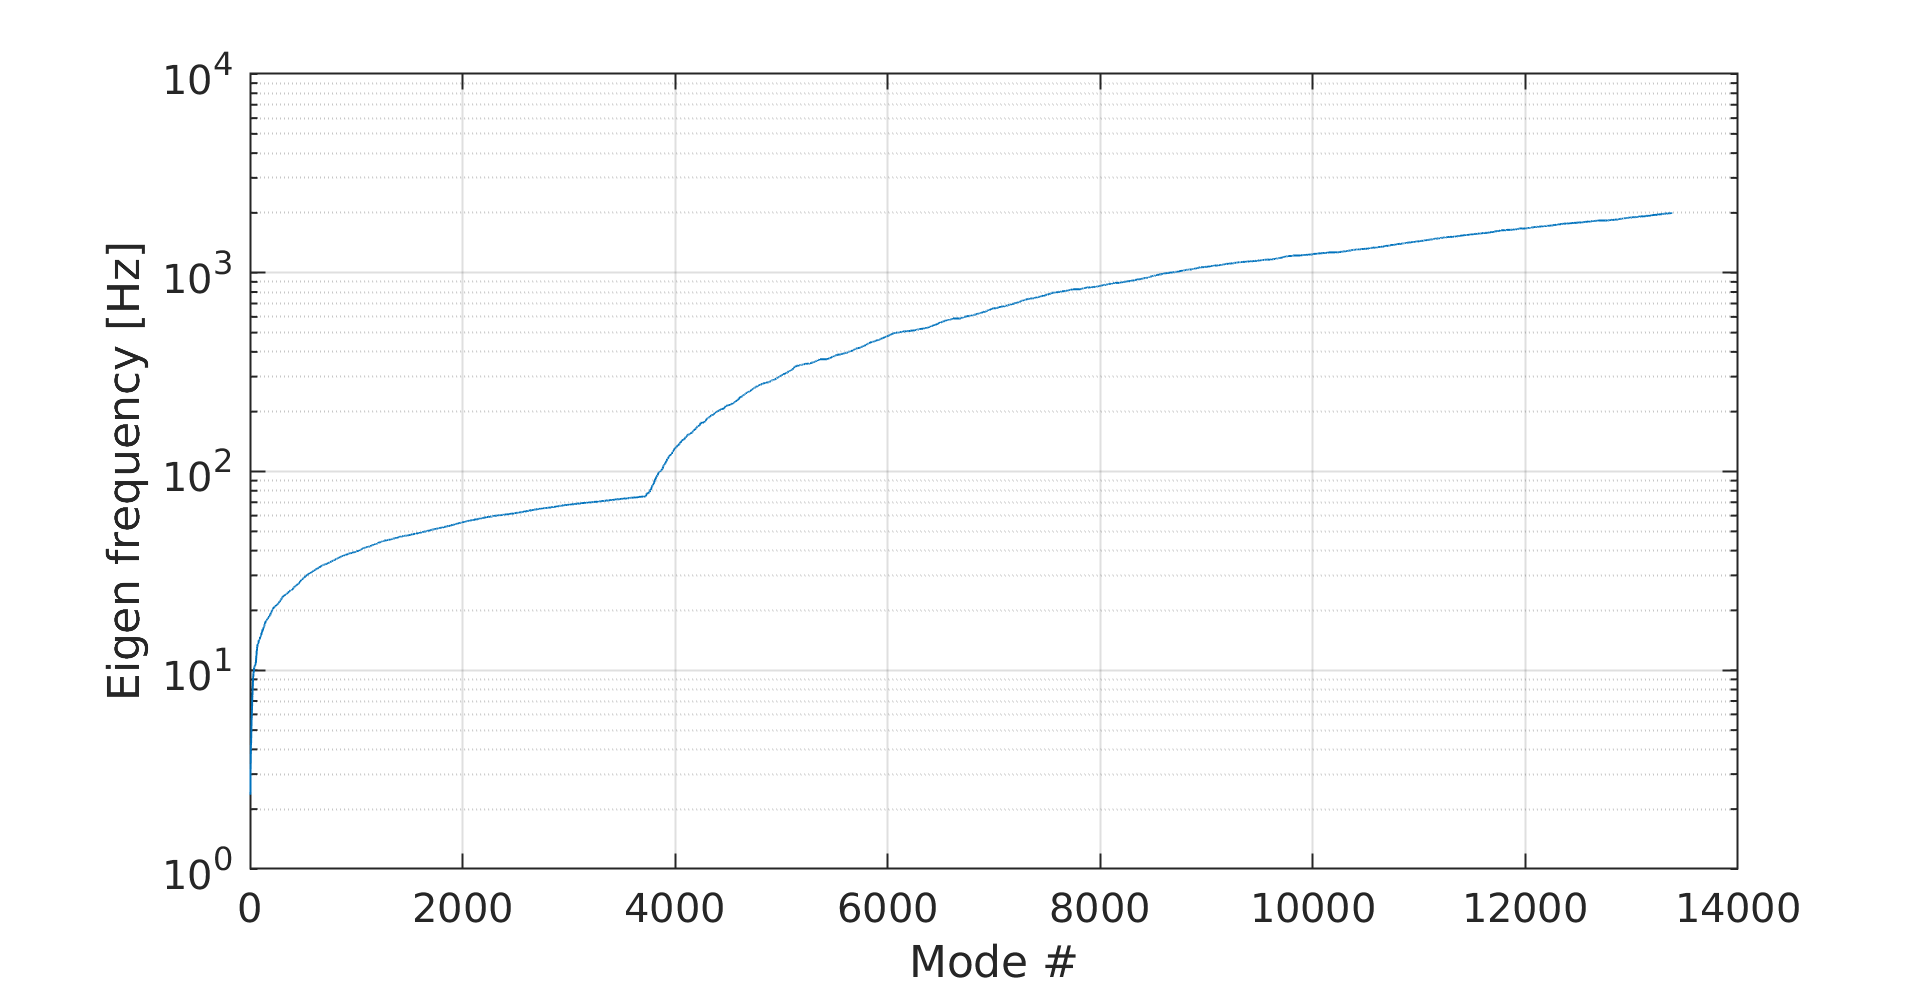
\includegraphics[width=0.7\linewidth]{modal_state_space_model_2ndOrder_2000Hz.png}
  \caption{Telescope FEM eigen frequencies as a function of the eigen modes
    number.}
  \label{fig:fem-eig-val}
\end{figure}
To reduce the computing burden, the number of modes of the system is reduced by
thresholding the Hankel singular values of the system.
The state space model is set with a modal damping coefficient $\zeta=2$\% and a
sampling rate $\tau=1$ms. 

A set of inputs and outputs are added to the FEM in order to apply
forces and moments to the model and to get the corresponding node displacements.
The inputs forces and moments are
\begin{description}
\item[the wind load forces](Sec.~\ref{sec:cfd}) applied to
  \begin{itemize}
  \item   the mount top-end, trusses, C-Ring and GIR,
  \item  M1 segment cells, mirrors and mirror covers,
  \item  M2 segments,
  \end{itemize}
\item[the mount drive torques] on the elevation, azimuth and GIR axes,
\item[M1] hardpoints and support actuator forces,
\item[M2] positionner and FSM actuator forces.
\end{description}
The outputs nodes displacements are
\begin{description}
\item[the mount encoder angles] of the elevation, azimuth and GIR axes,
\item[M1]
  \begin{itemize}
  \item hardpoint displacement,
  \item segment rigid body motions,
  \item segment surface deformations,
  \end{itemize}
\item[M2]
  \begin{itemize}
  \item positionner and FSM actuator displacements,
  \item segment rigid body motions,
  \item segment surface deformations,
  \end{itemize}
\end{description}

ODC model integration\cite{mount_pdr_iv}

FEM to state space model\cite{ss2fem_Christoph2020}

The FEM of the telescope is composed of the FEM of the mount, of M1 and of M2.
It has been configured for 3 elevation angles: 90, 60 and 30 degrees.

To add for each elevation angle:
\begin{itemize}
\item table of 1st few eigen frequencies
\item plot of modes vs. eigen frequencies
\item plot of modes vs. Hankel  singular values
\item plot of some transfer functions before and after model reduction
\end{itemize}


\subsubsection{Mount FEM}
\label{sec:mount-fem}

ODC\cite{}

\subsubsection{M1 FEM}
\label{sec:m1-fem}

\paragraph{Gravity support forces}

\paragraph{M1 eigen modes}

The telescope FEM in its state space representation provides as outputs the
displacement of nodes on the surface of M1 segments as well as the 6 rigid body
motions of the segments.
Both the surface deformations and the rigid body motions of the segments are
moved over to the optical model (Sec.~\ref{sec:optics}).
The optical model then updates the state of M1 segments before proceeding to ray
tracing through the telescope.

In the optical model, the surface deformations of the segments is superimposed
onto the rigid body motions i.e. the surfaces are defined in the coordinate system
associated to the rigid body motions whereas in the FEM the surfaces are defined with
respect to the coordinate system of each segment\cite{GMTO.CoordinateSystems}.

Assuming the vector of translation $\vec t_i$, the rotation matrix $R_i$ and the
coordinate vector of node $k$ $\vec n_{i,k}$ at the surface of M1 segment \#$i$, the following
geometric transformation is applied to the nodes
\begin{equation}
  \label{eq:7}
  \vec n_{i,k} \leftarrow R_i^{-1}(\vec n_{i,k}-\vec t_i).
\end{equation}
Based of the lateral stiffness of M1 mirrors, it is assumed that $\vec
n_{i,k}-\vec t_i \simeq [0,0,\delta_{z,k}]^T$ and Eq.~(\ref{eq:7}) simplifies to
\begin{equation}
  \label{eq:8}
  \vec n_{i,k} \leftarrow \delta_{z,k} \vec r_{i,3} 
\end{equation}
where $\vec r_{i,3} = [r_{i,13},r_{i,23},r_{i,33}]^T$ is the 3rd column of $R_i^{-1}$.
Further neglecting the lateral surface shears of the mirror, the surface
deformation of segment $i$ is finally written as
\begin{equation}
  \label{eq:8}
  S_i = [\delta_{z,k}r_{i,33}]^T,\forall k \in i.
\end{equation}

To reduce the amount of data that is given to the optical model, the surface
$S_i$ is projected on the M1 segment eigen modes $B_i$ like so $b_i = B_i^TS_i$
where $B_i$ is derived from the singular values decomposition of the sensitivity
matrix $F_i$ that relates actuator cylinder forces to surface deformations, $F_i
= U_i \Lambda_i V_i^T$.
The 6 lowest eigen values correspond to the 6 rigid body motions that have been
filtered out of each influence function in $F_i$ and $B_i$ is given by $U_i$
with the 6 eigen modes corresponding to the 6 lowest eigen values removed.

Using $B_i$ as the modal basis for M1 segments in the optical model, we can compute
a calibration matrix $D$ that relates the mode coefficients $b$ to the WFS
measurements $s$, $s=Db$.
The actuator forces are related to the modes coefficients with $f_i =
V_i\Lambda_i^{-1}b_i = V_i\Lambda_i^{-1}D^\dagger s$ and these forces must bear
no loads on the segments hardpoints as any hardpoints load would in turn induce
stresses into the glass.
It is worth noting that the feedback force measurements from the hardpoints load cells
would capture any spurious forces and off-load them to the actuators hence
``tainting'' the M1 surface deformations with hardpoint footprints.
In order to avoid such contamination from the hardpoint, a new segment modal
basis is derived in the following such as the associated forces lay in the null
space of the hardpoints.

The derivation starts from the gain $G$ of the FEM static solution reduced to M1
actuator forces as inputs and hardpoint displacements and M1 surface
deformations as outputs:
\begin{equation}
  \label{eq:9}
  G = \begin{bmatrix}
    G_\beta \\ G_\alpha
  \end{bmatrix},
\end{equation}
where $G_\beta$ and $G_\alpha$ are the gain matrices for the hardpoints and
mirror surface, respectively, from which we compute the singular value
decomposition:
\begin{eqnarray}
  \label{eq:10}
  G_\beta &=& U_\beta\Lambda_\beta V_\beta^T \\
  G_\alpha &=& U_\alpha\Lambda_\alpha V_\alpha^T .
\end{eqnarray}
Both $V_\beta$ and $V_\alpha$ are forces eigen vectors and the hardpoints forces
eigen vectors are filtered out of the mirror surface with
\begin{equation}
  \label{eq:11}
  \bar V_\alpha = V_\alpha - V_\beta V_\beta^T  V_\alpha.
\end{equation}
The hardpoints displacements corresponding to the actuator forces given by $\bar
V_\alpha$ are written
\begin{equation}
  \label{eq:12}
  G_\beta \bar V_\alpha = G_\beta  V_\alpha - G_\beta V_\beta V_\beta^T  V_\alpha = U_\beta\Lambda_\beta V_\beta^T V_\alpha - U_\beta\Lambda_\beta V_\beta^T V_\alpha =0,
\end{equation}
using the orthonormal property of the eigen vectors, $V^TV=I$.
The final eigen modes are given by the left eigen vectors $U$ of the newly
formed gain matrix $\bar G$,
\begin{equation}
  \label{eq:13}
  \bar G = \bar U_\alpha\Lambda_\alpha V_\alpha^T = U\Lambda V^T.
\end{equation}

\subsubsection{M2 FEM}
\label{sec:m2-fem}


\clearpage
\subsection{Optical model}
\label{sec:optics}

\cite{GMTO.OpticalDesign}

\subsubsection{GMT optical model}
\label{sec:gom}

plot of GMT pupil (M2 baffle (3.6m), M1 drain holes, trusses)

\paragraph{M1 polishing error}

\paragraph{M1 gravity print-through}

\subsubsection{AGWS model}
\label{sec:agws}

\paragraph{SH24}

\paragraph{SH48}



\clearpage
\subsection{Control Model Architecture}
\label{sec:control}

Fig.~\ref{fig:NS_end2end} illustrates the integrated modeling simulation setup for the Natural Seeing observation mode. %
%
\begin{figure}[!hbt]
    \centering
    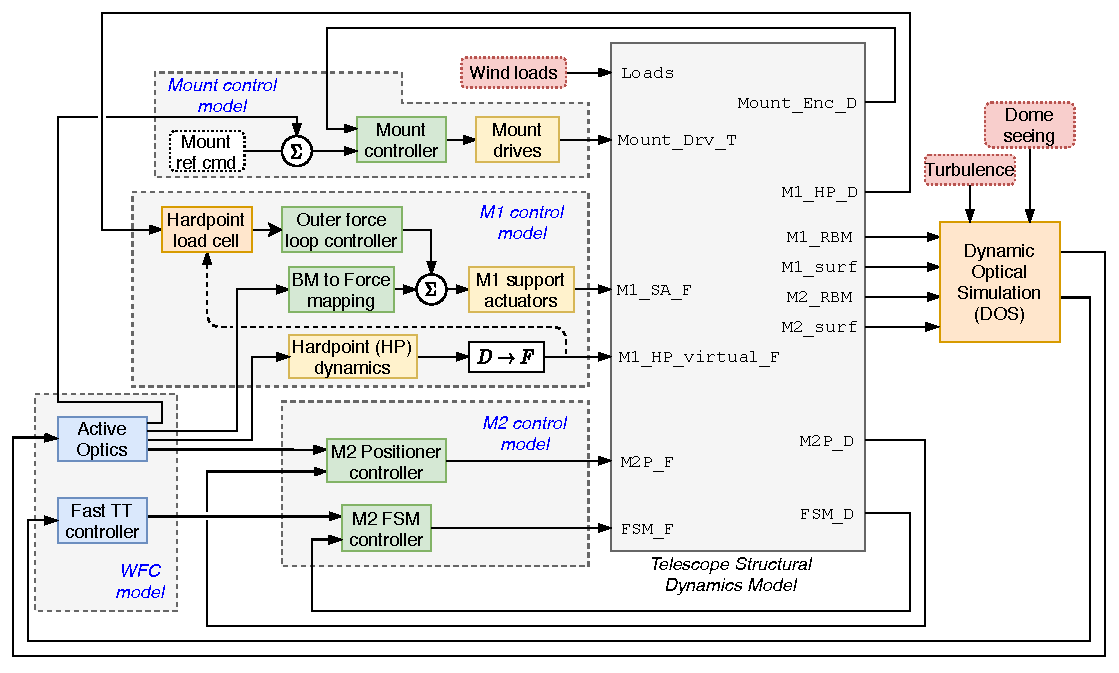
\includegraphics[width=\textwidth]{NS_end2end_syslevel.pdf}
    \caption{Natural seeing end--to--end simulation setup.}
    \label{fig:NS_end2end}
\end{figure}
%
 The telescope structural dynamics~\cite{ss2fem_Christoph2020}, the optical propagation block (DOS)~\cite{Conan2017_DOS}, and the control model compose the end--to--end simulation framework. One can split the control model into two groups: the wavefront control (WFC) and the local device/mechanical subsystem loops. The active optics and the segment tip--tilt (Fast TT) controller belong to the first group, relying on feedback from wavefront sensor measurements. The second has the lower--level control systems, namely the mount, M1 (outer force and position control), and M2 (Positioner and inner FSM loop controllers). In the following, we provide a brief description of each subsystem control model. For a complete presentation, one is referred to the indicated references.


\subsubsection{NS wavefront control system}
\label{sec:optics-ctrl}

Fig.~\ref{fig:ns-ctrl} reproduces the Natural Seeing OPM control block diagram from the GMT Observatory Architecture Document~\cite{OAD}. That diagram adds extra details wavefront control model, such as the interface of the controllers with the  Acquisition, Guiding and Wavefront Sensing (AGWS) unit and the commanded subsystems. The Natural Seeing algorithm description document~\cite{GMTO.NS.Alg.DOC} presents the wavefront control algorithms in more detail. This subsection provides a brief description of the wavefront controllers incorporated into the integrated modeling (IM) framework. 
\begin{figure}[!htb]
  \centering
  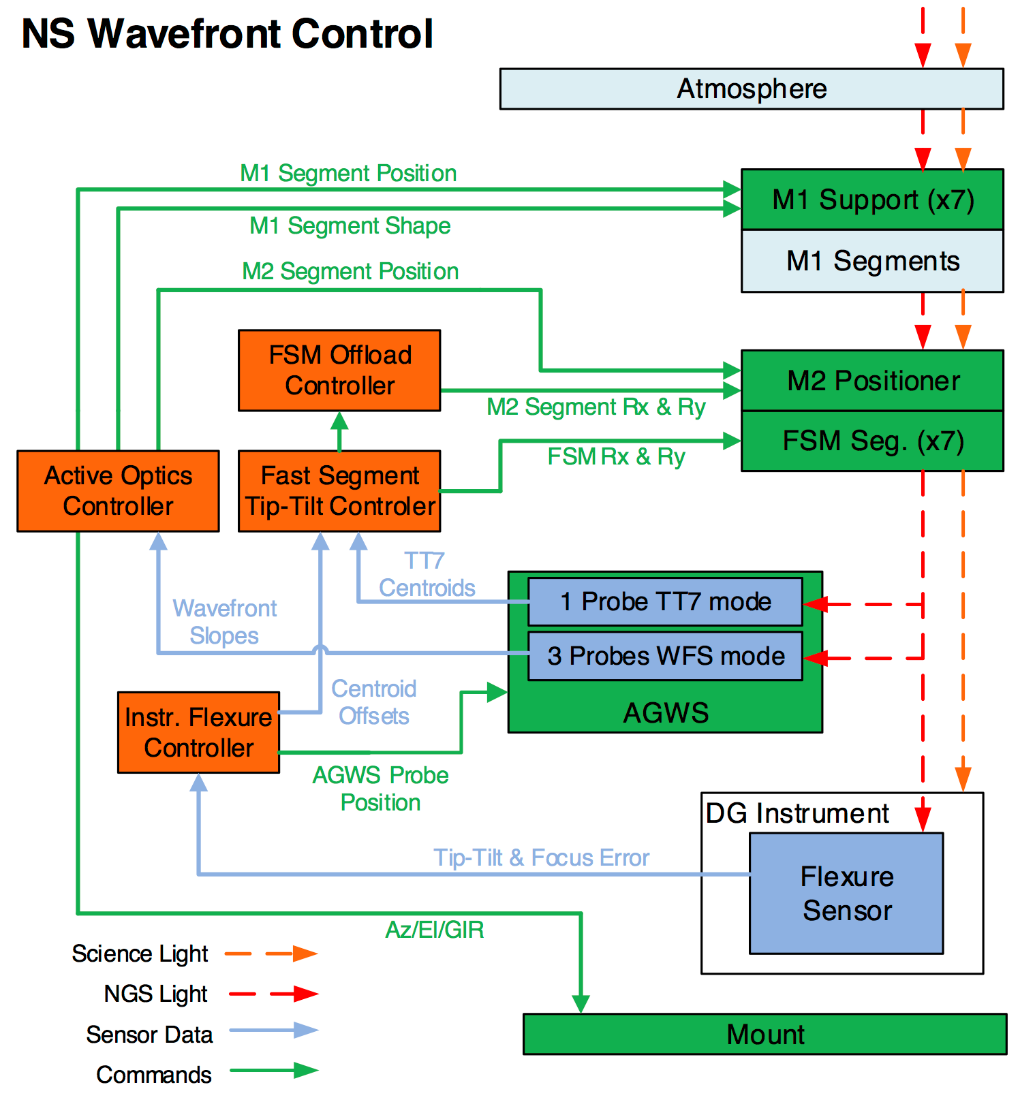
\includegraphics[width=0.7\linewidth]{ns-control.png}
  \caption{Natural Seeing wavefront control block diagram.}
  \label{fig:ns-ctrl}
\end{figure}


%\paragraph{Segment tip--tilt loop}

The Segment Tip--Tilt (Fast TT) Control Loop aims at minimizing image jitter by sending TT commands to the FSM. The feedback signal is the segment wavefront slopes measured by one of the four AGWS probes (in the TT mode that provides the slopes from a $24 \times 24$ lenslet array). The loop nominal frame rate is \SI{200}{Hz}. In the current design, the Fast TT controller has an integral controller connected to a lead--lag structure. The goal is to partially compensate for the lag of the inner FSM loop and also improve the disturbance rejection in the low--frequency range, without compromising the stability margins. Fig.~\ref{fig:ttt_s7_plots} depicts control loop characterization plots. On the left, the Nichols chart indicates that the considered design provides comfortable stability margins, as the open--loop responses do not approach the robustness boundary. On the right, one can see that the achieved sensitivity function is within the rejection transfer function (RTF) envelope, which is even more stringent than the nominal sensitivity defined in REQ--L3--OAD--35337 around \SI{10}{Hz}.
%
\begin{figure}[!htb]
  \centering
  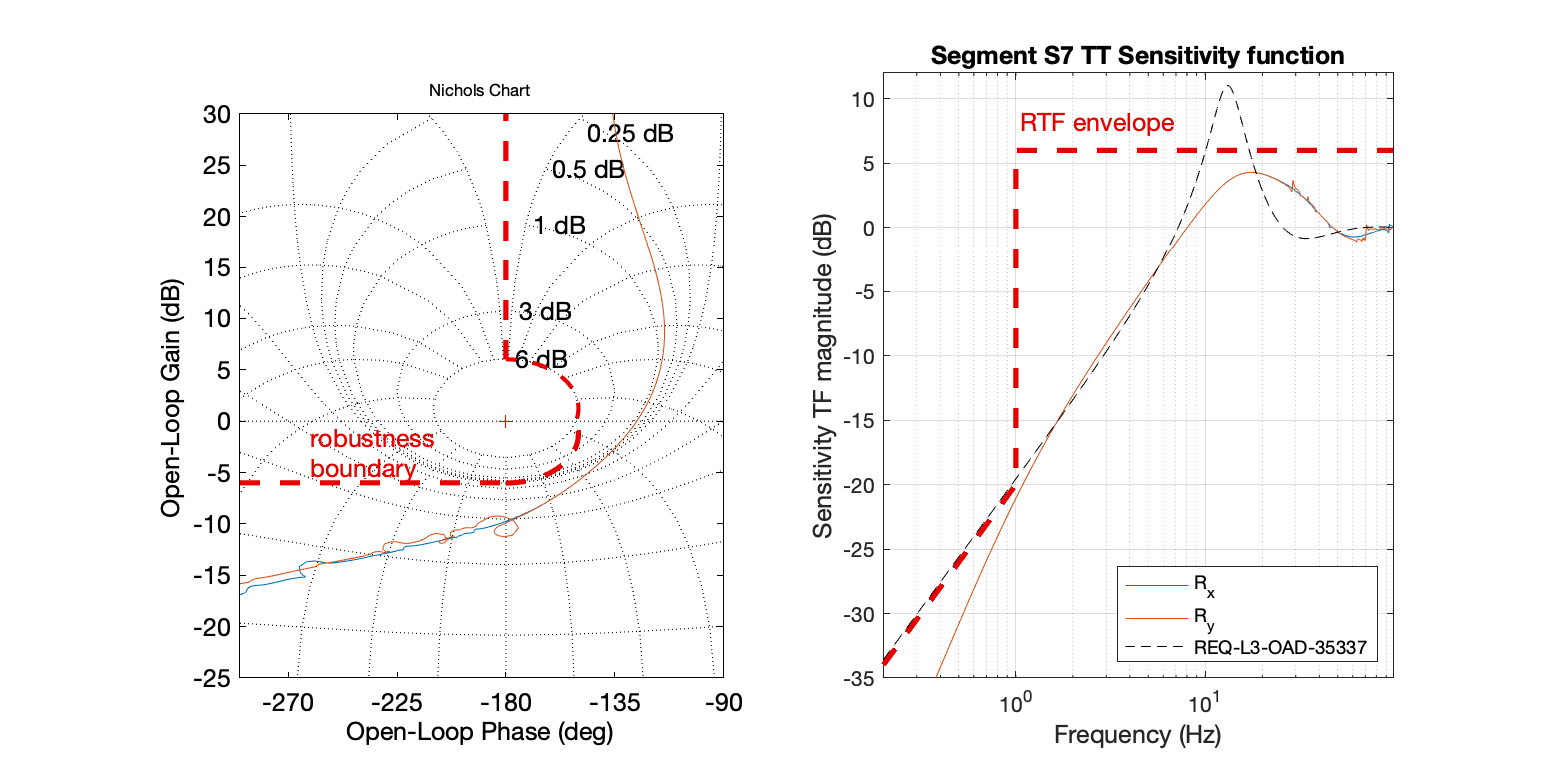
\includegraphics[width=\linewidth]{tt_S7_nichols_T.eps}
  \caption[Open-loop and sensitivity transfer function plots for the center segment.]{Open-loop and sensitivity transfer function plots for the center segment (S7).}
  \label{fig:ttt_s7_plots}
\end{figure}
The characterization plots for other segments and more details about the segment Tip--Tilt control model are presented in \cite[Section~4.3]{GMT.DOC.05154}.

%\paragraph{Active Optics}

The active optics (AcO) control strategy can be split into two steps. % (Fig. ???). 
First, there is an estimation (or reconstruction) step that aims at recovering the controllable modes (states) based on measurements of at least 3 AGWS probes in the WFS mode, such that each one provides the slopes from a Shack--Hartmann WFS with a $48 \times 48$ lenslet array. The controllable modes are the M1 and M2 rigid--body motions (RBMs), a subset of the M1 bending modes (BMs), and eventually global pointing errors projected onto azimuth (AZ), elevation (EL) and GIR axes. The active optics reconstruction is handled as an optimization problem based on four fundamental requirements: ({\it i}) wavefront error minimization, ({\it ii}) blind modes penalization --- piston error and outer--axis segment clocking, ({\it iii}) implementation of a load balance policy, and ({\it iv}) achieving an optimal solution within the admissible control set, that is, accounting for the actuator limits, which are imposed through inequality constraints. Second, a feedback integral compensator processes the reconstructed controllable modes and outputs correction commands to the M1 \& M2 segment position, the M1 shape and the mount orientation.

%\paragraph{FSM offload controller --- Include ?}
The FSM provides high bandwidth M2 segment $R_x$ and $R_y$ control with a limited range of motion, while the M2 Positioner provides lower bandwidth with a wider range of motion. The M2 Offload Loop (REQ--L3--OAD--34785~\cite{OAD}) aims at maximizing the available FSM stroke by maintaining the FSM actuators near the center of their range. The strategy described in~\cite[Section 6.4]{GMTO.NS.Alg.DOC} produces the FSM offloading signal by integrating the low--frequency trend of the segment tip--tilt corrections over a \SI{1}{s} time window. Such offloading contribution is summed to the AcO offset commands to the M2 positioned system.

The Instrument Flexure Control Loop aims at correcting differential flexure between the instrument and the AGWS using image motion and focus error measured by the instrument Flexure Sensor. That controller is not considered in the current version of the NS OPM.

\subsubsection{Mount controller}
\label{sec:mount-ctrl}

The mount structure shall follow a given trajectory that can be either slewing to a new science target in the sky or tracking a target. The controller ensures the mount stays on course while subject to various disturbances like the effects of gravity and wind buffeting. The mount controller generates compensation torque commands to the elevation, azimuth and Gregorian instrument rotator (GIR) drives axes to mitigate the tracking error computed based on the feedback signal of the mount axes encoders.  The mount control model also considers the drive actuators by representing their dynamics and some major nonlinear effects, such as quantization errors, friction, and parasitic torques.

Each mount axis is controlled independently using a PID compensator and resonance (notch) filters to cope with structural resonant modes. A feedforward strategy is also envisioned to relieve the feedback compensator during critical acceleration/deceleration phases. As illustrated in the mount controller frequency responses of Fig.~\ref{fig:mount-ctrl}, the filter parameters assume different tunings depending on the telescope elevation angle. %
\begin{figure}[!htb]
  \centering
  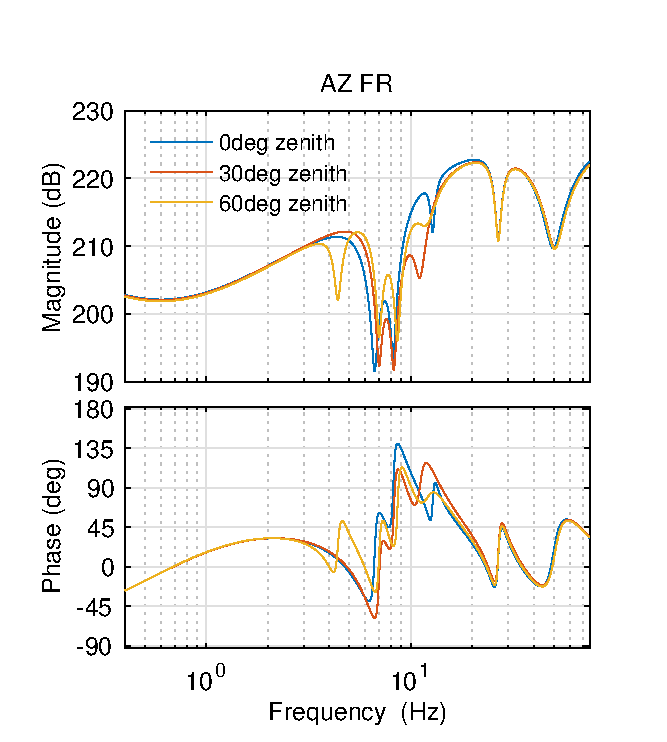
\includegraphics[width=0.32\linewidth]{AZ_fbC_za.eps}
    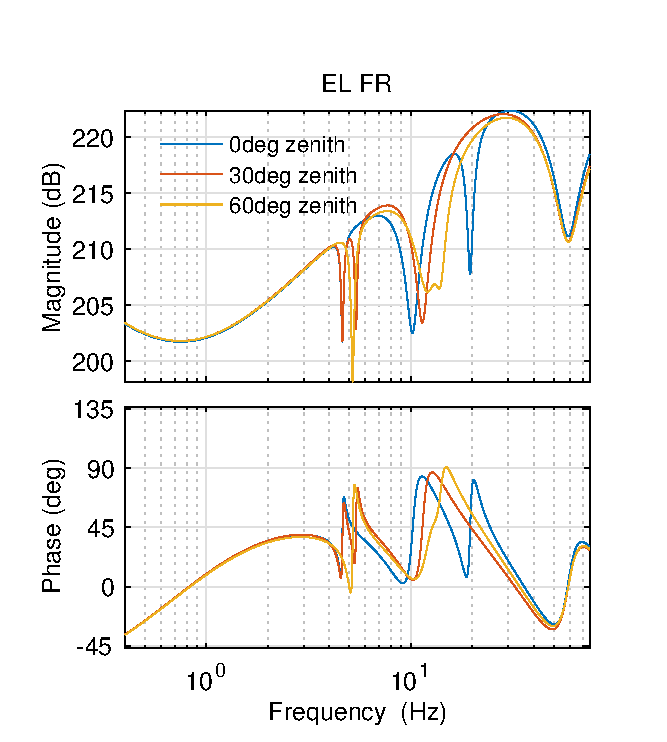
\includegraphics[width=0.32\linewidth]{EL_fbC_za.eps}
      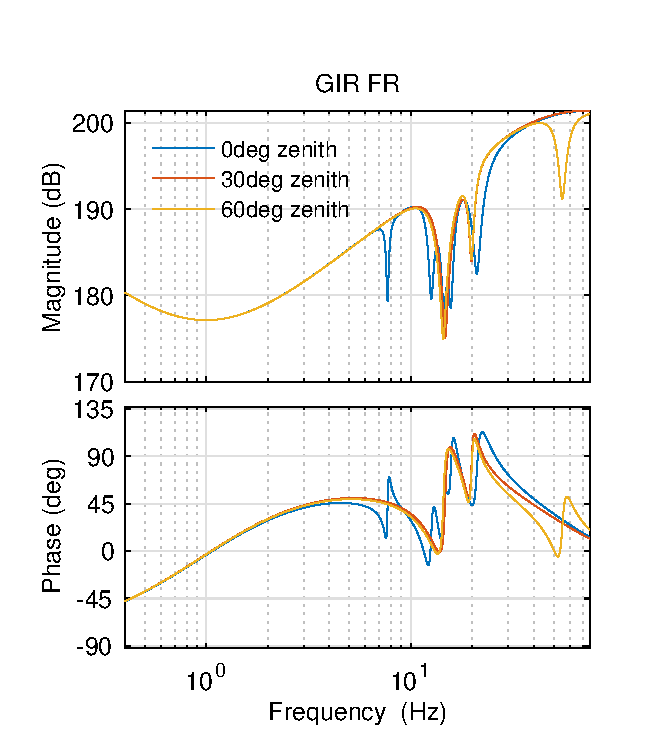
\includegraphics[width=0.32\linewidth]{GIR_fbC_za.eps}
  \caption{Mount feedback controllers for different elevation angles.}
  \label{fig:mount-ctrl}
\end{figure}
%
Fig.~\ref{fig:mount-cl-plots} shows the closed--loop (top) and sensitivity (bottom) frequency responses of each mount axis transfer function with the elevation structure at three different zenith angles. The considered structural damping is 2\%. %
\begin{figure}[!htb]
  \centering
  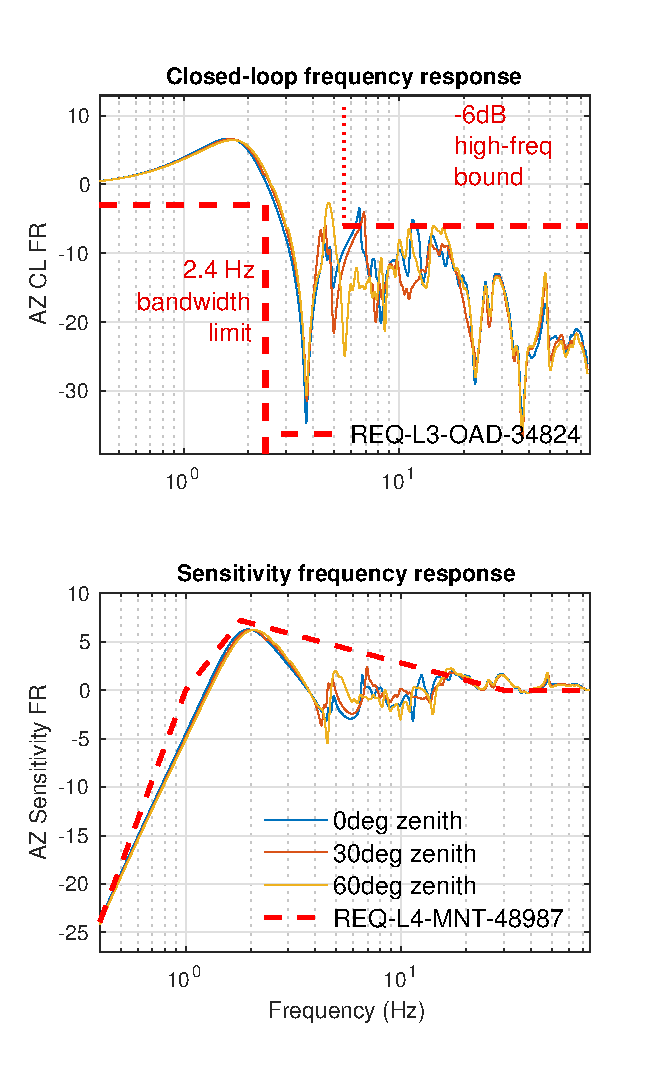
\includegraphics[width=0.32\linewidth]{az_CL_plots.eps}
    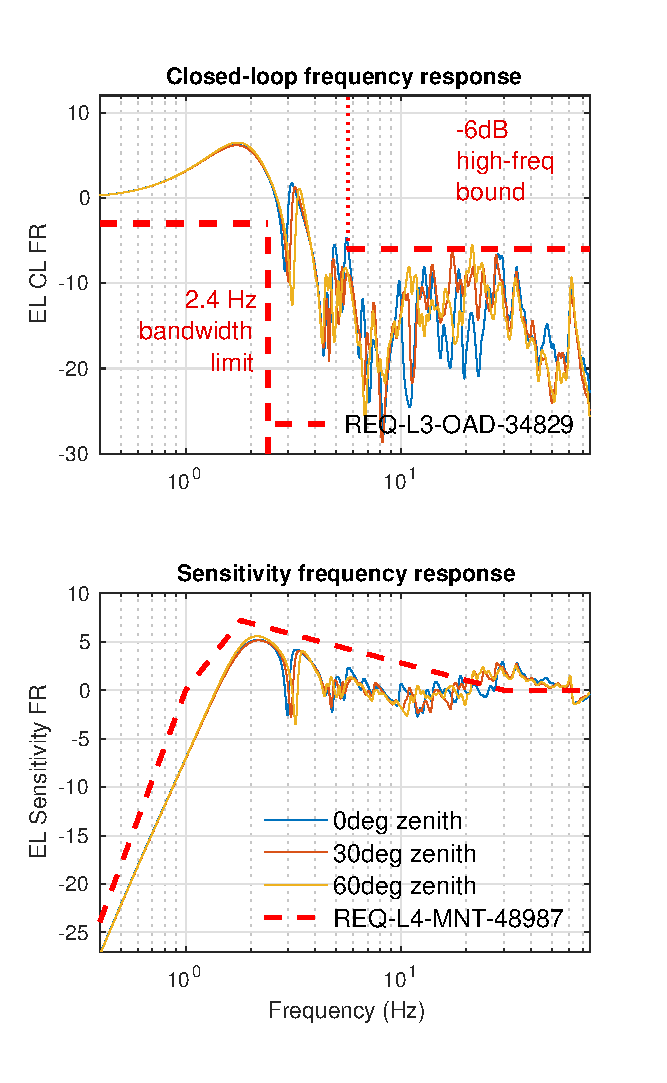
\includegraphics[width=0.32\linewidth]{el_CL_plots.eps}
      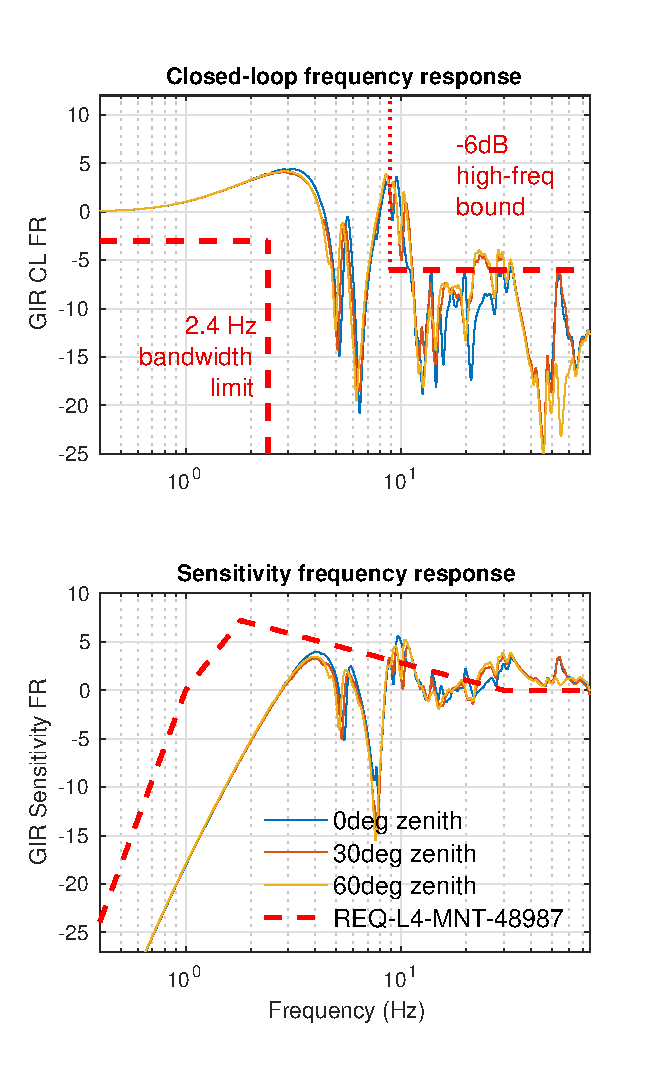
\includegraphics[width=0.32\linewidth]{gir_CL_plots.eps}
  \caption{Closed--loop and sensitivity frequency responses of the mount axes transfer functions.}
  \label{fig:mount-cl-plots}
\end{figure}
%
The OAD requirements REQ--L3--OAD--34824 and REQ--L3--OAD--34829 define a \SI{2.4}{Hz} closed--loop bandwidth for the azimuth and elevation axis, respectively. The red dashed lines indicate the envelope of complaint responses. The sensitivity plots include the rejection transfer function (RTF) limits REQ--L4--MNT--48987 stated in the Mount Requirement verification Methods~\cite[Section 5.6.1]{GMT.DOC.02011}. The results indicate that the OAD controller design achieves the required bandwidth. In addition, the obtained sensitivity transfer functions partially met RTF limits. Though the simulations suggest that the envelope violations at high--frequencies have not led to significant performance degradation, one should be aware of that issue. For convenience, the envelopes in the GIR plots (on the right) assume the same requirements as those used for the azimuth and elevation axes. The ODC GIR control design provides \SI{4.4}{Hz} bandwidth, significantly higher than the obtained for the other mount axes. The GIR loop disturbance rejection is also higher in the low--frequency range.

More details on the mount control model, including the structural dynamics behavior for different mount elevation angles, are reported in \cite[Section 3]{ODC_end2end_2021}.


\subsubsection{M1 subsystem local control}
%\subsubsection{M1 hardpoints to actuators force loop }
\label{sec:m1-ctrl}

Each primary mirror (M1) segment has six stiff actuators connected to the back of each segment, forming a hexapod. Those actuators (referred to as hardpoints, or simply HP) are also attached to the telescope mount through a cell weldment. Therefore, one defines the rigid--body position of the M1 segments by controlling the lengths of the hardpoints. In addition, the HPs have load cells mounted on the extremum of the actuator rods to measure the forces at the mirror attachment points.


A set of pneumatic actuators composes the M1 support system. Using the measurements of the HP load cells as feedback signals, the primary mirror device control system (M1DCS) commands the pneumatic actuators, which apply a force vector to the back surface of the mirrors. These pneumatic actuators can also provide axial compensation forces to correct mirror surface figure errors through the Active Optics (AcO) control loop.


Therefore, the role of the M1 control system is threefold. First, the primary mirror shall support the mirror segments while minimizing the stress at the connection points with the HPs. Second, controlling the shape of the primary mirrors. Third, to provide the reference position to each segment by commanding the lengths of the hardpoints. One of the goals of the integrated modeling effort is to develop end--to--end simulation models putting together the main telescope subsystems. To enable the evaluation of the effect of the M1 subsystem in the GMT optical performance, the simulation models incorporate the behavior of the hardpoints and the support actuator system. The document \cite{GMT.DOC.05153} discusses the M1 control under the GMT integrated model perspective.



\subsubsection{M2 subsystem control loops}
\label{sec:m2-ctrl}

Fig.~\ref{fig:fsm_control_arch} shows the secondary mirror (M2) control system model. The block diagram also indicates its interfaces with the segment TT and the active optics controller. %
%
\begin{figure}[!hbt]
    \vspace{6pt}
    \centering
    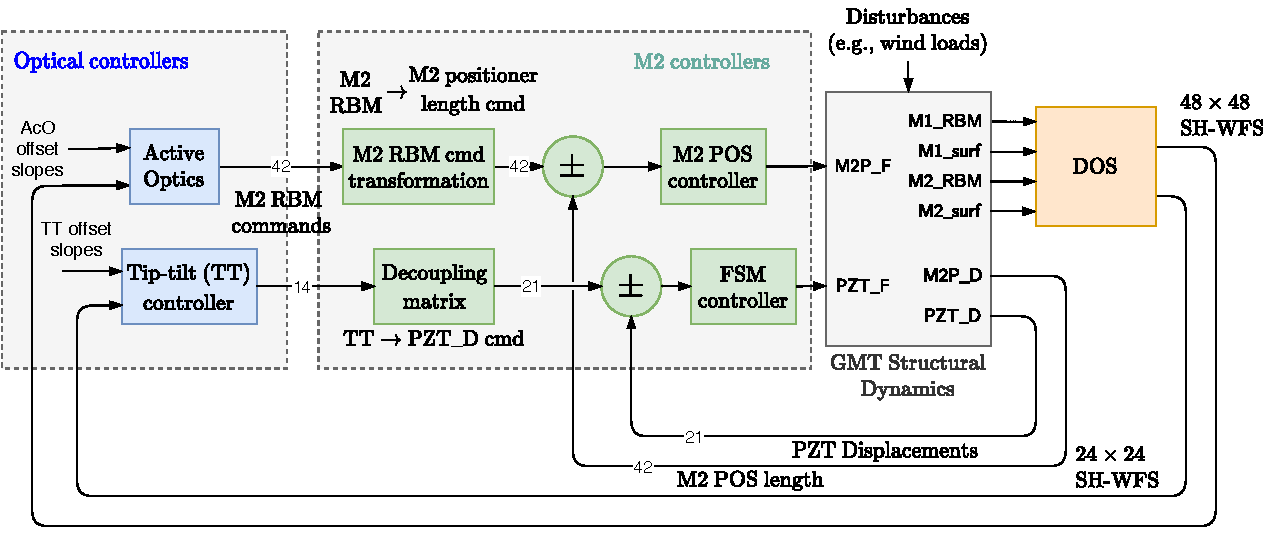
\includegraphics[width=\textwidth]{WFC-FSM_control_intf.pdf}
    \caption{M2 FSM control system architecture.}
    \label{fig:fsm_control_arch}
\end{figure}
%
%\paragraph{M2 positionner controller}
The M2 POS feedback controller takes the error vector of the positioner actuators lengths to calculate the respective control force signals. A $42 \times 42$--transformation matrix maps secondary mirror rigid-body motions, provided by the Active Optics Controller in the Natural Seeing Observing mode~\cite{GMTO.NS.Alg.DOC}, into the reference signal to the M2 positioner actuators lengths. The Observatory Requirement Document (OAD)~\cite{OAD}  stipulates through REQ--L3--OAD--35039 that the M2 positioner (M2P) shall provide a bandwidth of \SI{2}{Hz} while tracks the rigid--body motion commands.

%\paragraph{M2 segment piezo--actuators controller}
A decoupling matrix transforms the segment tip--tilt commands into linear positions references to the FSM piezo actuators (PZT), used as set--points to the FSM inner control loop (see Fig.~\ref{fig:fsm_control_arch}). By feeding back the differential displacements of the PZT actuators, the inner loop FSM controller provides actuator force commands to track the differential position command. %
The level--3 OAD requirement REQ--L3--OAD--35044 \cite{OAD} states that the dynamic response of the M2 FSMS shall be compatible with the one from a second--order linear system with a $0.6$ damping ratio and \SI{25}{Hz} bandwidth.


For a more detailed description of the M2 positioner and FSM inner controllers, including control loop robustness and performance analysis plots, one is referred to \cite[Section 4.1 and 4.2]{GMT.DOC.05154}.



\clearpage
\subsection{Disturbances}
\label{sec:disturbances}

\subsubsection{Atmospheric turbulence model}
\label{sec:atm}

validation of the atmospheric model\cite{GMT.DOC.01862}


\subsubsection{Computational fluid dynamics}
\label{sec:cfd}

\paragraph{Dome seeing}

\paragraph{Wind pressure}

\cite{GMTO.DOC.03352}

\subsubsection{M1 heat conjugate transfer model}
\label{sec:m1-hct}

\cite{GMT.DOC.04558,GMT.DOC.04557,GMT.DOC.04894}
\paragraph{Soak error}

\paragraph{Segment core thermal footprints}



\clearpage

\printbibliography

\end{document}
